\section{Second Member}


\subsection{Comments about the module}
FSE seems really useful. All of its merits are easily identifiable, at a glance one could list a multitude of them without even understanding the topic fully. The list would be so extensive that to recreate it would be to attempt such scripture on the scale of the copying of the various holy scripts, performed by the monks and priests across the western european countries in the middle ages. Perhaps, even, one could compare such epic amounts of detail to the hit folk book 'Potato and You', which goes into copious amounts of articulation for what is seemingly a dull and uninspiring topic.

\subsection{Selfie with Max}

\begin{figure}[h]
\caption{D U C K R O L L}
\centering
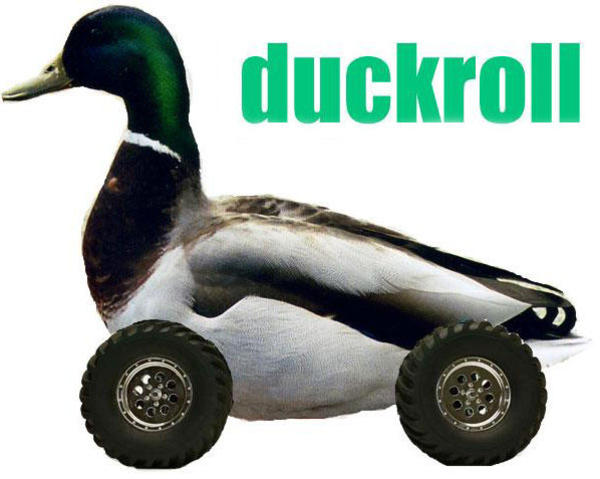
\includegraphics[width=0.5\textwidth]{Duckroll}
\label{fig:Duckroll in 2 0 1 7}
\end{figure}


% My selfie with Max is in  Figure~\ref{fig:selfie}.

\subsection{What I have learned in this module}
I have learned so much this module, from the minor, low impact intricacies to the major, groundbreaking discoveries, enlightening my mind to the greater developments in the software engineering process. 

